\vspace{-.2cm}
\section{Related Work}
\vspace{-.2cm}

\myparagraph{Transformers in Visual Learning.} Building upon the success of self-attention in language modeling, architectures that leverage transformer based token-mixing have been proposed for visual generation~\citep{parmar2018image,child2019generating,chang2022maskgit} and recognition tasks~\citep{ramachandran2019stand,cordonnier2019relationship}, cumulating in the ViT architecture which relies on very few locality biases~\citep{dosovitskiy2020image}. In the years since, many improvements and variants have been proposed~\citep{nauen2025transformer, vaswani2021scaling,tolstikhin2021mlp,bello2021lambdanetworks,tay2021synthesizer,touvron2021going}. The improvements have largely focused on data~\citep{pmlr-v139-touvron21a} and compute efficiency~\citep{tay2020sparse,choromanski2020rethinking,liu2021swin,ali2021xcit,roy2021efficient,zhou2021informer,yin2022vit,yao2022wave,liang2022not}. In general, vision transformers tokenize an image into a set of patches, where each patch is first processed using an MLP or convolution block~\cite{wu2021cvt,yuan2021tokens,chen2021visformer,chen2021crossvit}, the patches are further processed with self-attention which enables global token interactions beyond those in convolutional networks. As self-attention is permutation invariant, positional information is typically injected using learnable positional embeddings or relative positions~\citep{gehring2017convolutional, su2024roformer,fang2024eva,liu2021swin,lu2024fit,lu2024unified,kim2023region}. Positional embeddings have been suggested to play a role in the emergence of dense ViT artifacts, as networks with positional embeddings removed have smooth feature maps~\citep{yang2024denoising}.

\vspace{-.2cm}
\begin{figure}[t!]
  \centering
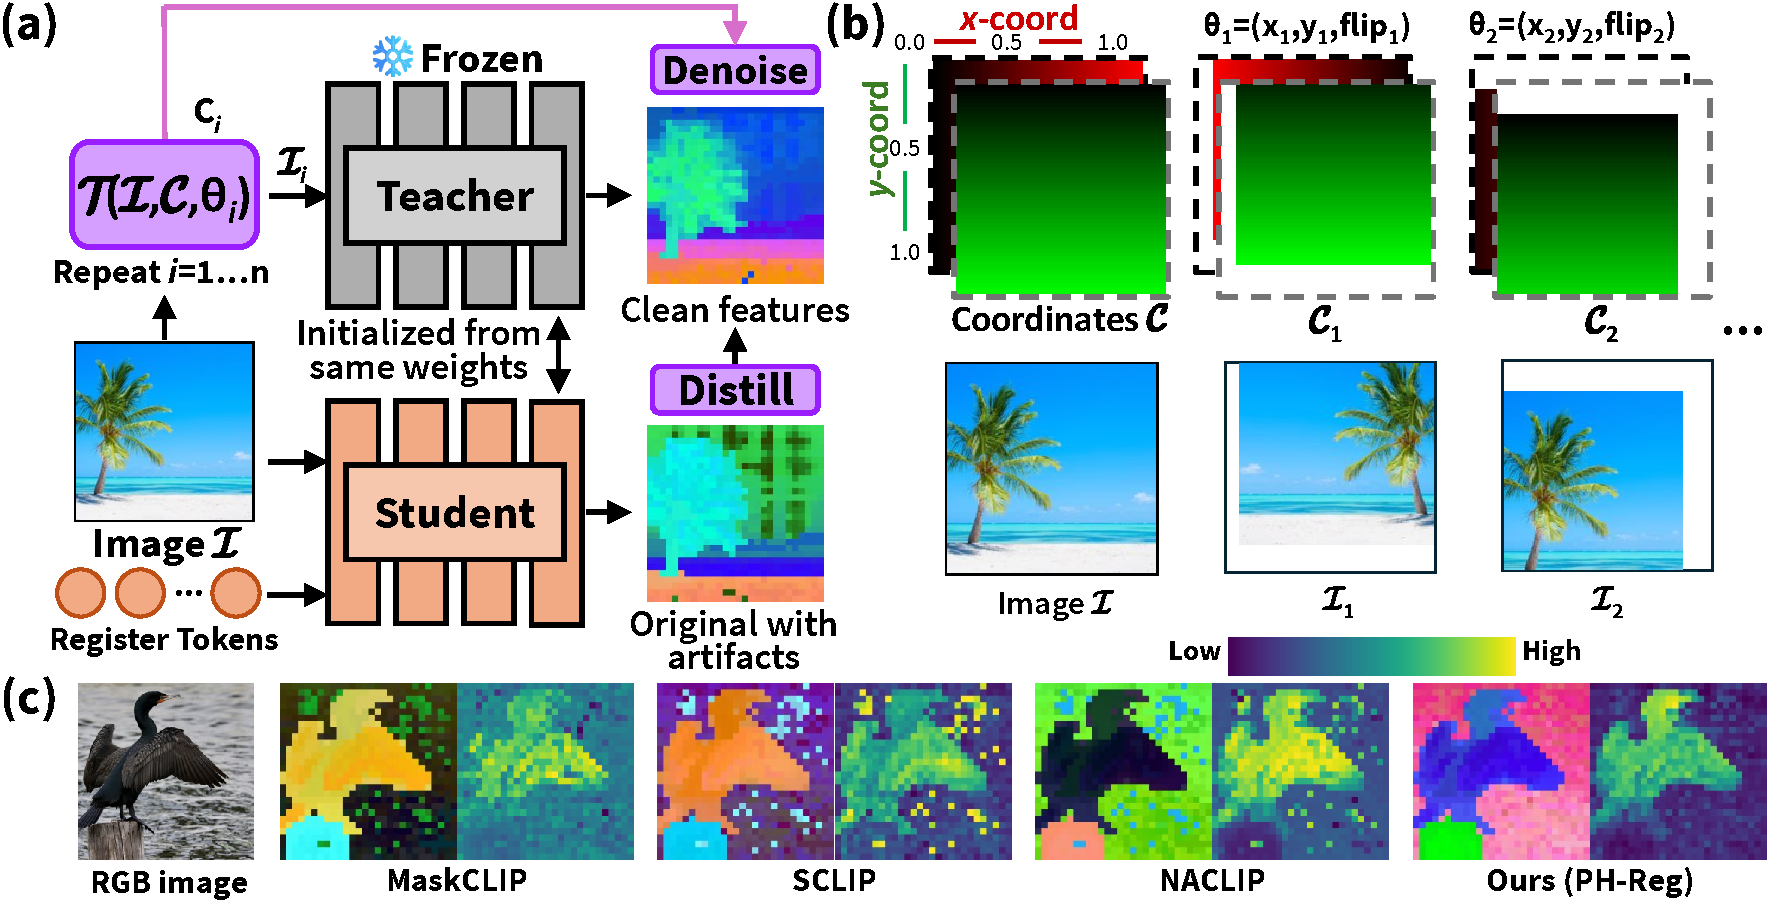
\includegraphics[width=1.0\linewidth]{fig_pdf/arch.pdf}
  \caption{\textbf{Learning Framework of PH-Reg.} \textbf{(a)} Our framework begins by creating two networks from the same set of weights. In the teacher, the weights are frozen and unmodified. In the student, the only additional parameters are learnable register tokens. The teacher creates a learning target using denoised representations. \textbf{(b)} An image $\mathcal{I}$ undergoes augmentation by function $\mathcal{T}$ with random augmentation parameters consisting of random offsets and horizontal flips.\textbf{(c)} Given an RGB image, we utilize UMAP to visualize the features, and a heatmap using CLIP text query. Our method can produce significantly cleaner dense representations with minimal additional inference cost.}
  \vspace{-.5cm}
  \label{fig:arch}
\end{figure}
\vspace{-.2cm}

\myparagraph{Representation Learning with Vision Transformers.} The lack of restrictive local inductive biases in Vision Transformers enables strong scaling behavior across a diverse set of tasks. Beyond traditional supervised learning on categorical datasets such as ImageNet, methods have been proposed to learn on large scale datasets by leveraging language contrastive objectives~\citep{Radford2021LearningTV,yu2022coca}, or self-supervised image-level objectives~\citep{caron2021emerging,chen2021mocov3,li2021esvit} and patch-level objectives~\citep{trinh2019selfieselfsupervisedpretrainingimage,pmlr-v119-chen20s,xie2021simmim,MaskedAutoencoders2021,zhou2021ibot,bao2022beit,assran2023self,oquab2023dinov2}. While the training objectives are very different, these methods enable strong zero-shot and linear-probe performance across a diverse set of tasks, suggesting that these methods effectively learn the \emph{underlying statistics} of visual input. While these methods lack explicit dense supervision, the dense features from these models have been shown to have strong zero-shot emergent behavior with language-based segmentation~\cite{zhou2022extract}, object part correspondence~\citep{amir2021deep}, and structural understanding~\citep{Ranzinger_2024_CVPR}.

\myparagraph{Artifacts in Vision Transformer Dense Features.} Recent work on DINOv2~\citep{oquab2023dinov2} has found that Vision Transformers can have artifacts in their dense features. It has been proposed that artifacts can be mitigated with ``register'' tokens~\citep{darcet2023vision,burtsev2020memory, xiao2023efficient, jiang2025vision}. These register tokens are effectively randomly initialized embeddings that are analogous to the \texttt{[CLS]} token. While registers participate in the self-attention process, they are discarded during output. This approach requires a model to be trained from scratch. The nature and the mechanisms that cause the emergence of artifact tokens are unclear, and there exists conflicting results on what information (global or no information) these artifact tokens contain~\citep{darcet2023vision,wang2024sinder}. Recent work has further investigated the mechanism of register tokens~\citep{lappe2025registerclstokensyield}. Our own results have found that artifact tokens are not necessarily high-norm, and can be low-norm as well. Unlike the observation by~\citep{yang2024denoising}, we find that positional embeddings alone cannot account fully for the artifacts. Regardless of ``why'' artifact tokens emerge, removing these artifacts is an active area of research, with proposals based on registers~\citep{darcet2023vision}, magnitude smoothness priors~\citep{wang2024sinder}, and the foundational work on leveraging neural fields to denoise ViTs with a static artifact component~\citep{yang2024denoising,yang2023emernerf, luo2024brain}. A concurrent line of work has sought to remove artifacts for open-vocabulary segmentation with training-free attention modifications~\citep{zhou2022extract, LI2025111409,wang2024scliprethinkingselfattentiondense,bousselham2023groundingeverythingemerginglocalization, lan2024clearclip, hajimiri2025naclip}. Our framework can be applied to existing pretrained networks, introduces  minimal additional parameters, can be applied to tasks beyond open-vocabulary segmentation, and makes no assumptions on the magnitude or static nature of the artifacts.
